%%%%%%%%%%%%%%%%%%%%%%%%%%%%%%%%%%%%%%%%%%%%%%%%% 
\section{Ciência de dados}

% Data science geral

%O dado não possui significado relevante e não conduz a nenhuma compreensão. Representa algo que não tem sentido a princípio. Portanto, não tem valor algum para embasar conclusões, muito menos respaldar decisões.

%A informação é a ordenação e organização dos dados de forma a transmitir significado e compreensão dentro de um determinado contexto. Seria o conjunto ou consolidação dos dados de forma a fundamentar o conhecimento.
Dados não possuem significado relevante por si só, tampouco conduzem a alguma compreensão ou embasam conclusões. Informação, por outro lado, é a ordenação e organização desses dados de forma a transmitir significado (\textit{i.e.} a consolidação dos dados a fim de fundamentar o conhecimento)\cite{dadosinfo2019diego}. 

Ciência de dados (ou \textit{data science} do inglês) significa o estudo científico da criação, validação e transformação de dados para criar significado (conhecimento). Cientista de dados é o profissional que usa de métodos científicos para criar significado a partir de dados ``crus'' \cite{dsa2013codeofconduct}.
Em outras palavras, o termo ciência de dados é um termo ``guarda-chuva'' que engloba as técnicas e ferramentas como inteligência artificial, aprendizado de máquina, processamento de linguagem natural, estatística, algoritmos, modelagem, simulação e qualquer outro método científico que gere significado a partir de dados estruturados e não estruturados \cite{survey}.

A Figura \ref{figura_as_seis_divisoes} resume as seis divisões da grande ciência de dados \cite{donoho201750}.

Estudos apontam que 80\% do tempo da ciência de dados é consumido na primeira etapa (ou divisão) \cite{donoho201750}. 
Esta etapa é essencial para o entendimento do contexto e problema relacionados aos dados a serem analisados, incluindo visualizações prévias dos valores de cada característica (\textit{feature}) e observações de estatísticas sobre os dados. 
A preparação (limpeza) e exploração fazem parte desta etapa, que é iterativa e não-exaustiva, isto é, precisa de atenção e refinamento contínuo até a conclusão do trabalho, independente do número de divisões envolvidas no processo.

\begin{figure}[ht]
    \caption{As seis divisões de Ciência de Dados \cite{donoho201750}}
    \centering % para centralizarmos a figura
    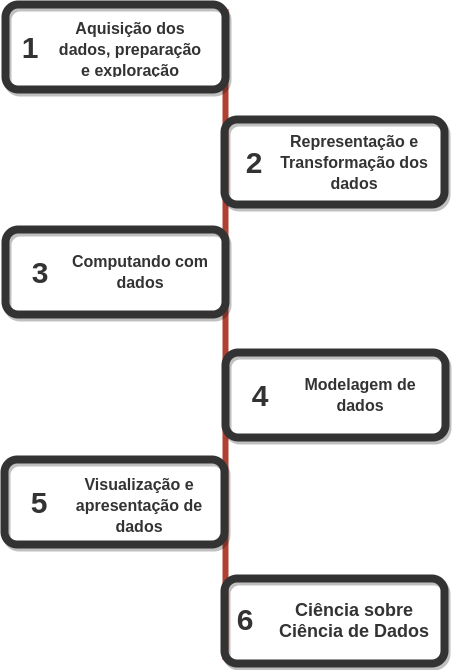
\includegraphics[width=8cm]{figuras/6divisoes_total.png}
    \label{figura_as_seis_divisoes}
    \end{figure}
    
%%%%%%%%%%%%%%%%%%%%%%%%%%%%%%%%%%%%%%%%%%%%%%%%% 
\subsection*{Aquisição dos dados, preparação e exploração}

\begin{enumerate}
        \item A \textit{aquisição dos dados} incorpora as diversas formas de coletar os dados, como planilhas no Excel, \textit{web scraping}, PubMed \textit{scraping}, processamento de imagem e manuseio de redes sociais como Twitter, Facebook e Reddit.
      
        \item A \textit{preparação} é necessária pelo fato de diversos conjuntos de dados conterem anomalias. 
        Todo projeto baseado em dados (\textit{i.e.}, \textit{data-driven}) requer uma busca minuciosa para identificar e corrigir anomalias, como dados faltantes, dados preenchidos erroneamente, dados inconsistentes e pontos fora da curva.
        Há erros frequentes de codificação em bancos de dados que podem levar a análises equivocadas dos dados, como foi o caso dos dados do censo indiano, cujas análises mostravam números excessivamente grandes de viúvas adolescentes  \cite{coale1962case}. 
        Esse tipo de erro pode ocorrer em qualquer cenário, ainda mais quando são utilizadas fontes não-estruturadas como blogs e tweets, ou até mesmo bases de dados alimentadas manualmente. 
        Esta preparação dos dados, para resolver problemas relacionados a anomalias, é uma subdivisão conhecida como limpeza e manipulação de dados (ou \textit{data cleaning} e \textit{data wrangling}) \cite{donoho201750}.
         
        \item Atualmente, é senso comum na área de ciência de dados que a \textit{exploração} é uma das atividades da análise de dados \cite{tukey1977exploratory} que mais demanda tempo dos profissionais da área. Essa fase é necessária para o entendimento do problema, e baseia-se em estudos univariados, bivariados, multivariados, limpezas básicas e testes de hipótese.
        O profissional responsável pela exploração precisa entender o contexto e a origem dos dados e utilizar recursos computacionais que facilitem a análise, uma vez que esta pode ser uma tarefa árdua ou inviável, principalmente se for feita sobre um grande volume ou variedade de dados. 
        Para ajudar no processo exploratório, existem ferramentas e técnicas (\textit{e.g.} Excel / planilhas; linguagens de programação: Python e R, com suas bibliotecas para processamento e visualização de dados -- pandas, numpy e matplotlib; Tableau) que permitem ao cientista de dados obter estatísticas e métricas do conjunto de dados. 
        As estatísticas fornecem uma visão geral dos dados, entendimento dos tipos das variáveis que pode ser utilizada para guiar a etapa de análise propriamente dita.
        Esta fase de exploração resulta, geralmente, em \textit{insights} cruciais aos trabalhos orientado a dados.
        \end{enumerate}

%%%%%%%%%%%%%%%%%%%%%%%%%%%%%%%%%%%%%%%%%%%%%%%%% 
\subsection*{Representação e Transformação dos dados}

    \begin{enumerate}
        \item A \textit{representação} dos dados é fundamental para resolver questões relacionadas à dados de entrada em formatos não-estruturados (\textit{e.g} fotografias, vídeos, áudios, registros financeiros, \textit{logs}, etc.), o que pode levar a um crescimento exponencial em complexidade de manipulação. 
        A criação de estruturas que forneçam uma representação (ou resumo) desses dados pode contribuir de sobremaneira na extração de \textit{insights} ou no armazenamento em padrões de representação para análises futuras.
                  
        \item A \textit{transformação} refere-se aos processos que convergem em uma reestruturação dos dados a partir das fontes originais. 
        Em outras palavras, o objetivo da transformação é, partindo de um estado complexo e ilegível dos dados originais, apresentar os dados em novos formatos e estruturas que facilitem a análise e a geração de \textit{insights}.
        
    \end{enumerate}
        
%%%%%%%%%%%%%%%%%%%%%%%%%%%%%%%%%%%%%%%%%%%%%%%%% 
\subsection*{Computando com dados}
Considerando o panorama mundial atual, onde dados são gerados com velocidades, variedades e volumes exponenciais, é vital que, além de conhecimentos estatísticos e matemáticos, o cientista de dados domine técnicas e tecnologias modernas de programação e computação, como manipulação de \textit{clusters} (\textit{e.g.} Apache Hadoop) e ferramentas de computação em nuvem (\textit{e.g.} Amazon AWS; Microsoft Azure).
    
%%%%%%%%%%%%%%%%%%%%%%%%%%%%%%%%%%%%%%%%%%%%%%%%% 
\subsection*{Modelagem de dados}
Modelagem descritiva, ou análise descritiva/exploratória é uma forma de utilizar ferramentas, métricas e técnicas estatísticas simples ou avançadas, para entender e explicar como os dados são. A análise descritiva é o processo mais básico para entender e responder a questões importantes como: ``qual a taxa de infecção da doença ao longo do ano?''.

Além desse tipo de modelagem, também é utilizada a modelagem preditiva. Esta serve para construir métodos que tentam prever um determinado cenário considerando um universo de dados, como o aprendizado de máquina moderno e seus desdobramentos industriais.
     
%%%%%%%%%%%%%%%%%%%%%%%%%%%%%%%%%%%%%%%%%%%%%%%%% 
\subsection*{Visualização e apresentação de dados}
As visualizações vão além de gráficos simples como histogramas, gráficos de dispersão e séries temporais. 
Os cientistas de dados, geralmente, investem um tempo significativo editando gráficos simples com cores, símbolos e anotações adicionais pra trazer um fator novo e importante sobre aqueles dados. 
Além disso, criam \textit{dashboards} para monitorar os \textit{pipelines} de processamento de dados e desenvolvem visualizações para apresentar conclusões de uma modelagem ou para responder alguma questão específica sobre os dados.
     
%%%%%%%%%%%%%%%%%%%%%%%%%%%%%%%%%%%%%%%%%%%%%%%%% 
\subsection*{Ciência sobre ciência de dados}
A ciência sobre ciência de dados diz respeito à identificação de fluxos de trabalho de análise ou processamento de dados. 
Por exemplo, pesquisas sobre melhorias dos processos de trabalho padrão, considerando fatores como tempo, recursos computacionais, confiabilidade da análise ou outras métricas de desempenho. 
Como um segundo exemplo, elaboração de documentação dos processos de análise de dados e conclusões individuais em formatos digitais para meta-análises futuras.

\section{Inteligência Artificial}
É um campo de estudo da computação que abrange uma enorme variedade de subcampos, onde tenta não somente compreender agentes inteligentes, mas também descrevê-las e implementa-las computacionalmente. Estuda os processos relacionados ao pensamento e raciocínio humano, tentando simular comportamentos que buscam agir e pensar como humanos ou racionalmente \cite{russell2004inteligencia}. 

\subsection{Aprendizagem de Máquina}
A aprendizagem de máquina (\textit{Machine Learning} - ML) é uma ramificação da Inteligência Artificial que estuda o desenvolvimento de técnicas e algoritmos para a construção de modelos preditivos.
Um modelo, por sua vez é simplesmente a especificação de uma relação matemática existente entre variáveis distintas. \cite{grus2019data}\cite{grus2019data}.
De modo geral, ML é uma automatização de modelos analíticos, que permitem o reeconhecimento de padrões ou realizar predições; dado um conjunto de treinamento, um algoritmo de ML é capaz de tomar decisões baseando-se em experiências adquiridas desse conjunto \cite{Monard2003a}. 

Os algoritmos e modelos de ML foram inspirados no processo de aprendizado humano, isto quer dizer que eles aprendem de modo iterativo com os dados, e permite que o próprio modelo encontre também, informações ou padrões ocultos nesses dados \cite{Monard2003a}.

\subsubsection**{Tipos de aprendizagem de máquina}
O aprenizado de máquina é realizado de três formas: (a) supervisionado, (b) não-supervisionado e (c) por reforço \cite{Monard2003a}.

\begin{enumerate}
    \item \textbf{Aprendizado supervisionado} -- Neste é dado ao algoritmo, uma base de conhecimento onde o estado final é conhecido. Literalmente, o modelo será ensinado sobre o que deve ser feito.
    Em outras palavras, um conjunto de dados rotulados é fornecido para o modelo, a fim de que este aprenda o que é cada classe/categoria.
    \begin{itemize}
        \item \textit{Classificação} -- é o método de predição de uma classe discreta ou categoria. 
        
        \item \textit{Regressão} -- é o método de predição de um valor contínuo.
    \end{itemize}
    
    \item \textbf{Aprendizado não-supervisionado} -- O algorítmo tenta formar agrupamentos a partir do seu próprio conhecimento. Diferente do aprendizado anterior, neste o conjunto de dados é não rotulado, e não ensina-se ao modelo qual o objetivo final. Esse tipo de aprendizado é baseado em busca e reconhecimento de padrões e relacionamentos.
    
    \begin{itemize}
        \item \textit{Agrupamento} (\textit{clustering}) -- esse método busca a similaridade entre os dados e, após identificar, segrega os itens entre os grupos específicos.
        
        \item \textit{Associação} -- utilizado quando se tem uma sequência de algo e deseja-se encontrar padrões.
        
        \item \textit{redução de dimensão} -- processo de redução da quantidade de variáveis aleatórias, a fim de se obter um conjunto de variáveis principais em consideração.
    \end{itemize}

    \item \textbf{Aprendizado por reforço} -- O objetivo desse tipo de aprendizado, é encontrar um modelo de ação adequado que maximize a recompensa acumulada total do agente.
    
\end{enumerate}

\subsubsection*{Árvore de Decisão}
Esse classificador é estruturado no formado de uma árvore binária, e apresenta possíveis caminhos de decisão e um resultaddo para cada caminho. São ligeiramente simples de interpretar e acompanhar o fluxo para uma previsão, além da possibilidade de se trabalhar com atributos numéricos e categóricos \cite{grus2019data}.

\begin{figure}[ht]
\caption{Modelo genérico de uma árvore de decisão.}
\centering % para centralizarmos a figura
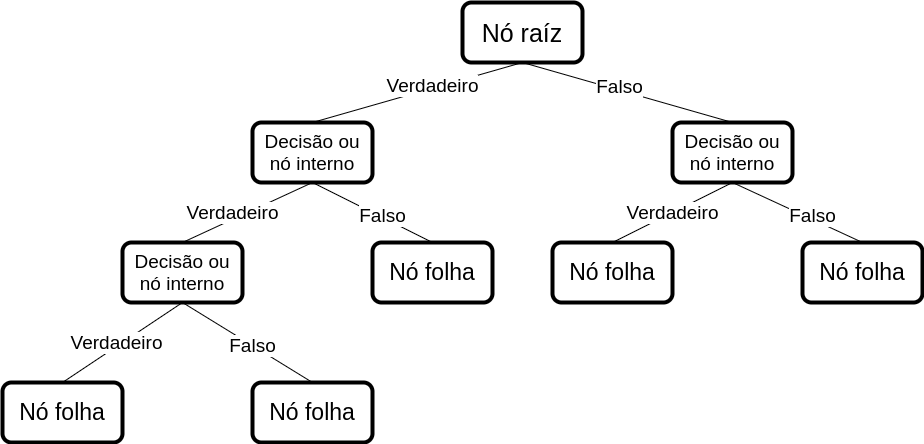
\includegraphics[width=15cm]{figuras/arvore_decisao.png}
\label{figura_arvore_decisao}
\end{figure}

A figura \ref{figura_arvore_decisao} apresenta um modelo genérico do funcionamento do método de árvore de decisão. O \textit{Nó Raiz}, presente no início da árvore corresponde à aplicação de um teste binário (\textit{Verdadeiro} ou \textit{Falso}). O fluxo segue dentre os \textit{Nós Internos}, que também os classificam através de testes binários, iterativamente, até chegar em um \textit{Nó folha}, onde econtra-se a classificação feita pela árvore \cite{russell2004inteligencia}.

\subsubsection*{Floresta aleatória}
Esse algorítmo é uma combinação de árvores de decisão, na maioria dos casos, treinados com o métoddo de \textit{bagging}. A premissa do método \textit{bagging} é que a combinação (\textit{ensemble)} dos modelos de aprendizado aumenta o resultado geral.
Quando uma árvore de decisão é construída, ela difere de uma outra árvore que utilizou dados diferentes ou ordem diferente para ser criada, pois se ajustam conforme seus dados de treinamento. A floresta aleatória (\textit{Random Forest}) permite, então, que várias árvores de decisão sejam criadas e decidam como classificar sua entrada. \cite{grus2019data}

\subsubsection*{Perceptron Multicamadas}
A perceptron multicamadas (\textit{MultiLayer Perceptron - MLP}) é uma rede neural com mais de uma camada de neurônios artificiais em alimentação direta. Esse tipo de rede é composta por camadas de neurônios interligados por sinapses com seus respectivos pesos de ativação (peso sináptico) \cite{russell2004inteligencia}.
O processo de aprendizado nesse tipo de rede, geralmente é feito através do algoritmo \textit{backpropagation} \cite{haykin2007redes}.

\subsubsection*{Validação de classificação}
Para medir e validar o desempenho de um classificador binário, é necessário primariamente separar uma porção dos dados para teste e para validações. Com isso, existem métricas de validação que buscam avaliar o quão bom o classificador é. Neste trabalho, utilizaremos as seguintes métricas:

\textbf{Matriz de Confusão --} é usada para se obter uma visão mais ampla ao avaliar o desempenho de um modelo.

\begin{figure}[ht]
\caption{Representação do modelo conceitual de uma Matriz de Confusão \cite{amidi2020ml}}
\centering % para centralizarmos a figura
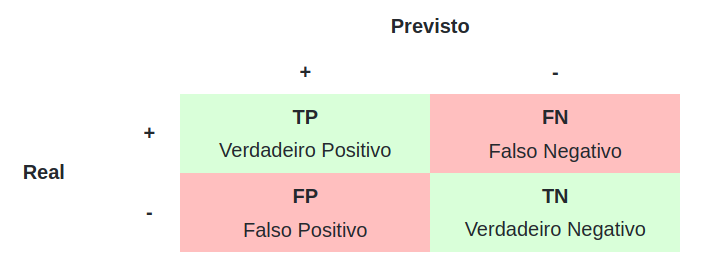
\includegraphics[width=12cm]{figuras/matriz_confusao.png}
\label{figura_matriz_confusao}
\end{figure}

A Figura \ref{figura_matriz_confusao} representa o modelo da matriz, onde \textit{Verdadeiro Positivo} -- TP denota os casos positivos previstos corretamente; \textit{Falso Positivo} -- FP para casos positivos previstos como negativos; \textit{Falso Negativo} -- FN é uma classificação oposta ao FP; \textit{Verdadeiro Negativo} -- TN para casos corretamente classificados, porém inversos ao TP \cite{amidi2020ml} .

\begin{table}[htb]
\centering 
    \caption{\textbf{Métricas de avaliação}}
    \label{tab:metricas}
    \vspace{2mm}
%\resizebox{\columnwidth}{!}{%
    \begin{tabular}{| l| c | c | }
    \hline
    \textbf{Métrica} &\textbf{Fórmula} &\textbf{Interpretação}\\ \hline
    Acurácia & $\frac{TP + TN}{TP + TN + FP + FN}$ &Desempenho geral do modelo \\ \hline
    Precisão & $\frac{TP} {TP + FP}$ & Quão precisas são as previsões positivas \\ \hline
    Sensibilidade & $\frac{TP} {TP + FN}$ & Cobertura da amostra positiva real \\ \hline
    Especificidade & $\frac{TN} {TN + FP}$ & Cobertura da amostra negativa real \\ \hline
    F1 score & $\frac{2 TP} {2 TP + FP + FN}$ & Métrica híbrida útil para classes não balanceadas \\ \hline
    \end{tabular}
    %}

\end{table}

A partir da matríz de confusão, as extrae-se as métricas de avaliação: Acurácia, Precisão, Sensibilidade, Especificidade e F1 score, descritos na Tabela \ref{tab:metricas}.

\textbf{ROC e AUC --} \textit{Receiver Operating Charactgeristic} e \textit{Area Under the Curve}, onde um gráfico mostra a curva correspondente da Sensibilidade pela Especificidade (ROC). Este gráfico resume todas as matrizes de confusão que cada limiar produziu, ajudando a decidir qual dos modelos gerados pelas matrizes é o mais adequado. A área abaixo da curva (AUC) representa o grau de separabilidade da curva, descrito no intervalo de 0 a 1. Sendo 1 o modelo perfeito, e 0 o menor valor, no qual o modelo errou todas as classificações dos dados.
